O campus do Gama da Universidade de Brasília, construído entre os anos de 2009 a 2011, localizado na Área Especial de Indústria Projeção A, UnB - Setor Leste Gama, Brasília-DF, possui área total de 335074 $m^2$, com área construída de 16009 $m^2$, sendo projetada para abrigar no total, cinco cursos de engenharia, sendo eles de Aeroespacial, Automotiva, Eletrônica, Energia e Software.

\begin{figure}[H]
  \centering
  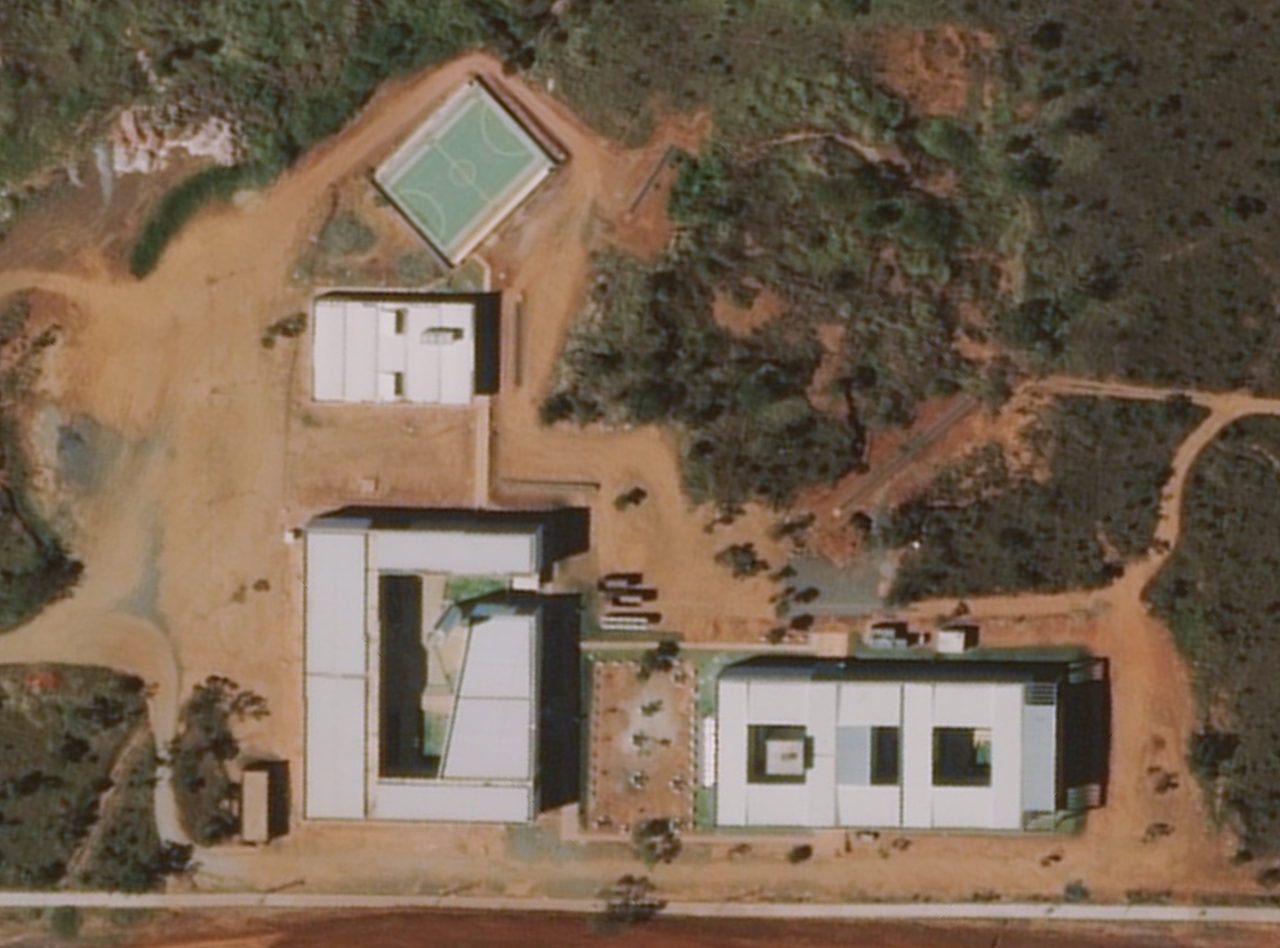
\includegraphics[width=0.87\textwidth]{figuras/fga1}
  \caption{Vista aérea do campus UnB Gama. Em destaque os prédios já construídos.}
  \label{img:fga1}
\end{figure}

Contudo, algumas partes da obra envolvendo a segurança, como cercamento e monitoramento de quem entra e quem sai não foram concluídas, colocando em risco a integridade física e dos bens daqueles que frequentam o núcleo de ensino. Como maneira de averiguar o fluxo de circulação das pessoas no local, foi elaborada uma pesquisa envolvendo  92 alunos da Faculdade do Gama [figura \ref{img:pesquisa}], onde cerca de 41\%  utilizam automóveis para se deslocarem até o mesmo.

\begin{figure}[H]
  \centering
  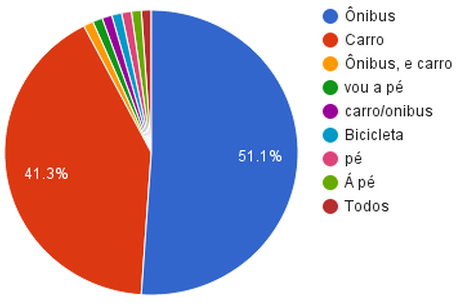
\includegraphics[width=0.75\textwidth]{figuras/pesquisa}
  \caption{Pesquisa de mobilidade dos alunos da FGA. Fonte: Do autor, 2015.}
  \label{img:pesquisa}
\end{figure}

De acordo com os dados coletados na pesquisa, entre o período de 2010 a 2015, 13 roubos foram computados, mas apenas 10 registros oficiais, como boletins de ocorrências, foram registrados. Dessa maneira, há a necessidade de se projetar  um sistema que possa realizar o monitoramento  da área do estacionamento e fluxo de pessoas  com o objetivo de aumentar o controle de entradas e saídas de veículos e pessoas no campus. Além disso, tal sistema também contribuiria para a proteção das fronteiras do campus, já que o território é grande e em maior parte desocupado.
